
\section{Deliverable 6: Evasion attacks}

\textcolor{red}{\textbf{For all of the attacks, I have attached the ipynb notebook that has all the runs for the TAs to see}. The file is called attacks.ipynb}

\subsection{Task 1 (Untargeted) vs Task 2 (Targeted)}


\begin{solve}

I am only showing this for one image here, but tried for a set of three images and the results were similar.

The plots of purturbed images and the original images are shown below for both the tasks. The success rate and accuracy plots are also shown for both the models.

Note that the success rate for Untargeted attacks just means that there was misclassificaiton, whereeas for Targeted attacks, it means that the attack was successful in making the model predict the target class (in our case our class that we want to attack was 1 and we wanted the model to predict 8). 

We see that for epsilon .02 and .05 it is hard to see the difference between the original and the purturbed images, but for epsilon .1, the difference is visible. We start seeing artificats.

Note that in the case of targeted attacks, we used PGD. Given the value of $\alpha = .0392$, we see that the attack is quite visible even for $\epsilon \sim .04$


\textbf{Model A vs Model B for Targeted and Untargeted Attacks}
\begin{itemize}
    \item For Untargeted attacks, the success rate is higher for Model B than Model A, it remains constant for Model B, but changes for Model A.
    \item For Targeted attacks, the success rate is higher for Model A than Model B. Infact we are unable to get any successful attack on Model B even with very high $\epsilon$ values as compared to Model A for the same $\alpha$ values.
    We also see that the test accuracy does not change for model B dyring the attack, showing that not only we are failing in targeted attacks but we are also not able to misclassify the images in untargeted sense.
    This shows that Model B is more robust to targeted attacks than Model A in this setting.
    \item It might be that Model B is specifically trained to be robust to such targeted attacks, or it might be that Model B is more robust to such attacks in general. We cannot say this until we do tets on other kinds of targeted attacks and not just on $1$ and $8$ clases.
\end{itemize}


\subsubsection{Untargeted Attack}

\begin{figure}[H]
    \centering
    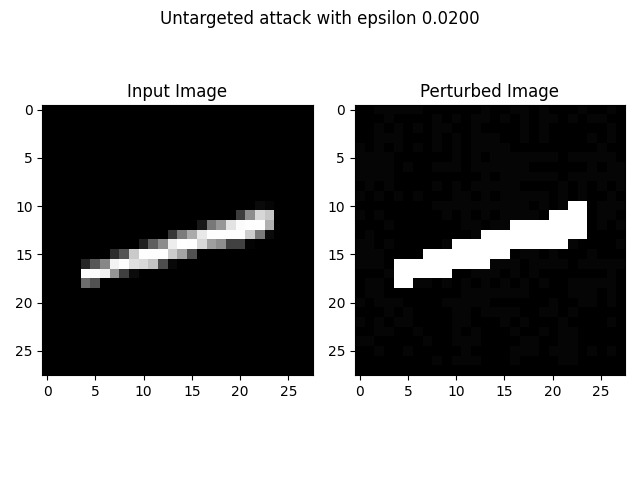
\includegraphics[trim={0 1.5cm 0cm 0}, width=.5\textwidth]{/Users/vashisth/Documents/GitHub/Intro_DL/IDL_HW3/HW3_tex/plots/Del6/Untargeted/Untargeted_attack__modA_0.0200_Img-2.png}
% \end{figure}
% \begin{figure}[H]
    \centering
    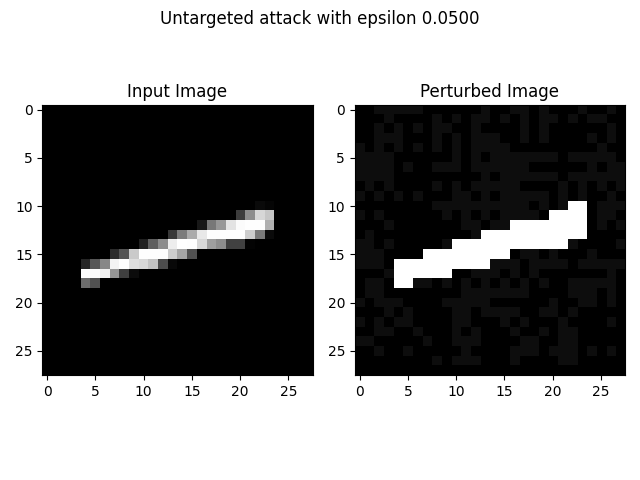
\includegraphics[trim={0 1.5cm 0cm 0}, width=.5\textwidth]{/Users/vashisth/Documents/GitHub/Intro_DL/IDL_HW3/HW3_tex/plots/Del6/Untargeted/Untargeted_attack__modA_0.0500_Img-2.png}
% \end{figure}

% \begin{figure}[H]
    \centering
    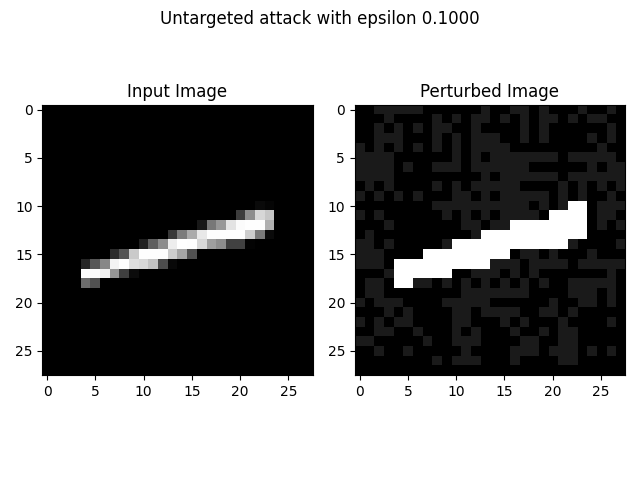
\includegraphics[trim={0 1.5cm 0cm 0}, width=.5\textwidth]{/Users/vashisth/Documents/GitHub/Intro_DL/IDL_HW3/HW3_tex/plots/Del6/Untargeted/Untargeted_attack__modA_0.1000_Img-2.png}
    \caption{Untargeted Attack on Model A for Image with index 2 for different $\epsilon$}
\end{figure}
% [width = .99\textwidth]


\begin{figure}[H]
    \centering
    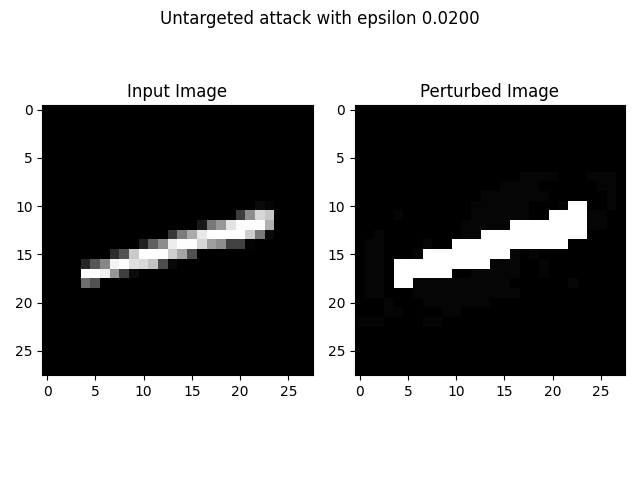
\includegraphics[trim={0 1.5cm 0cm 0}, width=.5\textwidth]{/Users/vashisth/Documents/GitHub/Intro_DL/IDL_HW3/HW3_tex/plots/Del6/Untargeted/Untargeted_attack__modB_0.0200_Img-2.png}
% \end{figure}
% \begin{figure}[H]
    \centering
    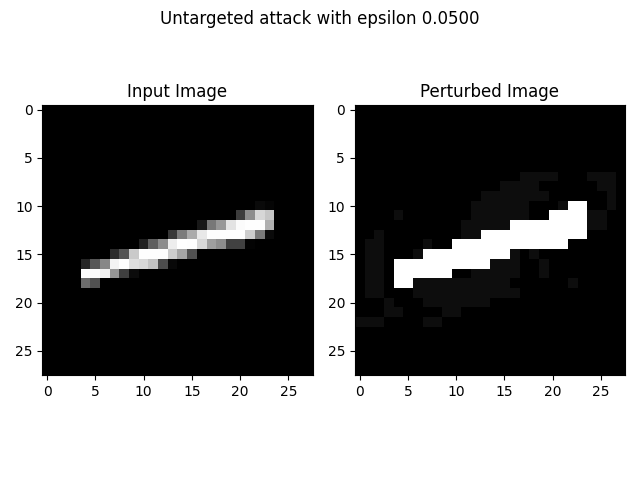
\includegraphics[trim={0 1.5cm 0cm 0}, width=.5\textwidth]{/Users/vashisth/Documents/GitHub/Intro_DL/IDL_HW3/HW3_tex/plots/Del6/Untargeted/Untargeted_attack__modB_0.0500_Img-2.png}
% \end{figure}

% \begin{figure}[H]
    \centering
    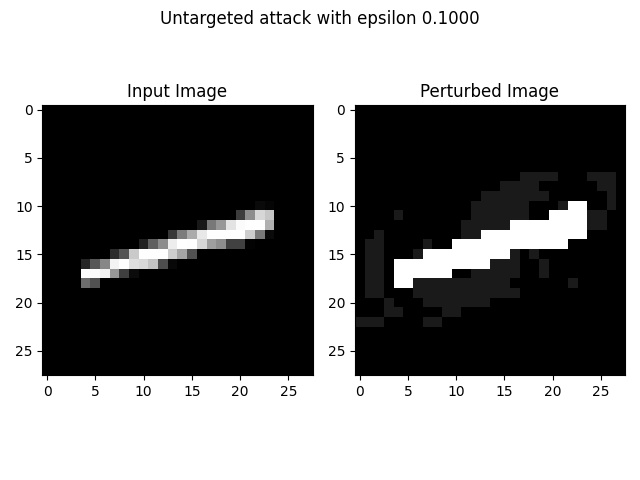
\includegraphics[trim={0 1.5cm 0cm 0}, width=.5\textwidth]{/Users/vashisth/Documents/GitHub/Intro_DL/IDL_HW3/HW3_tex/plots/Del6/Untargeted/Untargeted_attack__modB_0.1000_Img-2.png}
    \caption{Untargeted Attack on Model B for Image with index 2 for different $\epsilon$}
\end{figure}

\begin{figure}[H]
\centering
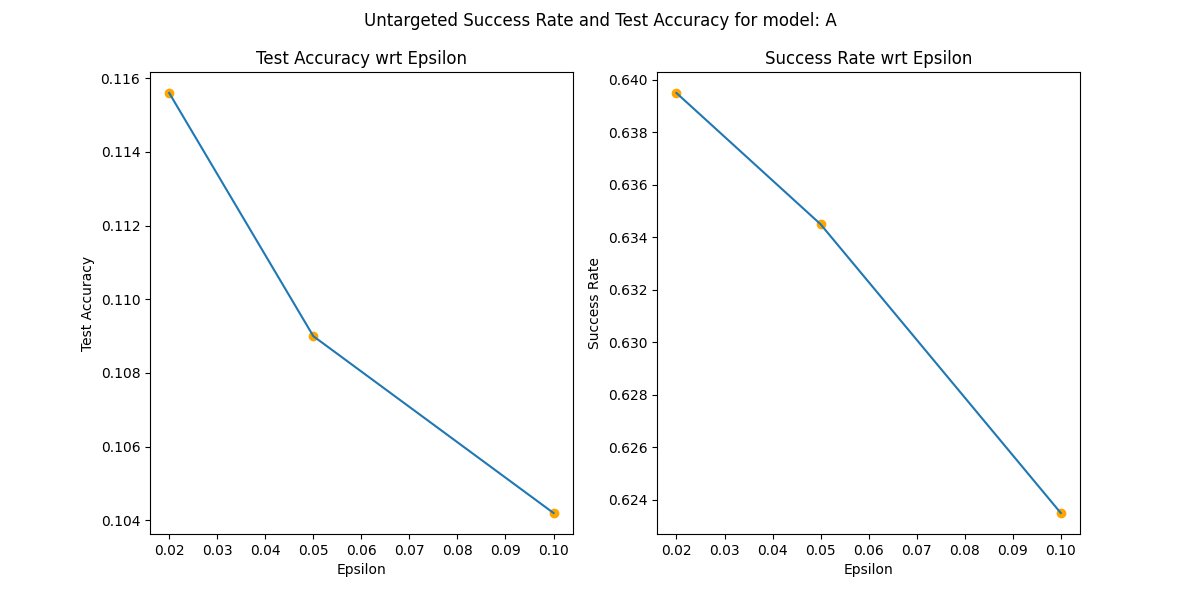
\includegraphics[width = .6 \textwidth]{/Users/vashisth/Documents/GitHub/Intro_DL/IDL_HW3/HW3_tex/plots/Del6/success_rate_plot_Untargeted_modA.png}
\caption{Success Rate and Accuracy Plot for Untargeted Attack on Model A}
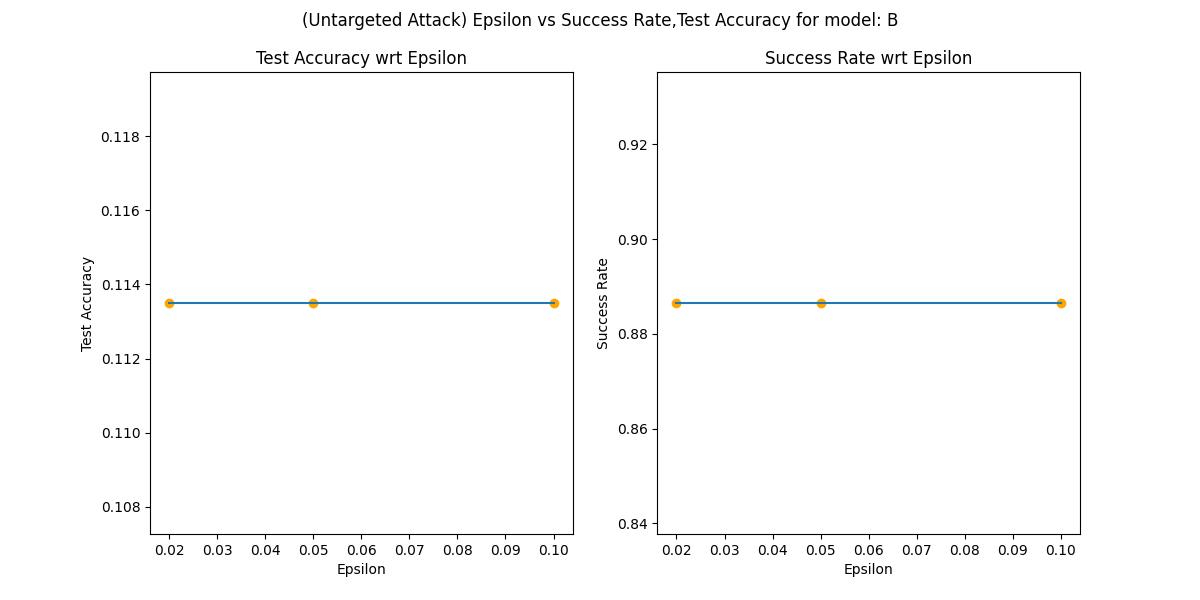
\includegraphics[width = .6 \textwidth]{/Users/vashisth/Documents/GitHub/Intro_DL/IDL_HW3/HW3_tex/plots/Del6/success_rate_plot_(Untargeted Attack)_modB.png}
\caption{Success Rate and Accuracy Plot for Untargeted Attack on Model B}
\end{figure}

% \end{solve}


%%%%%%%%%%%%%%%%%%%%%%%%%%%%%%%%%%%%%%%%%%

\subsubsection{Targeted Attack}

% \begin{solve}
\begin{figure}[H]
    \centering
    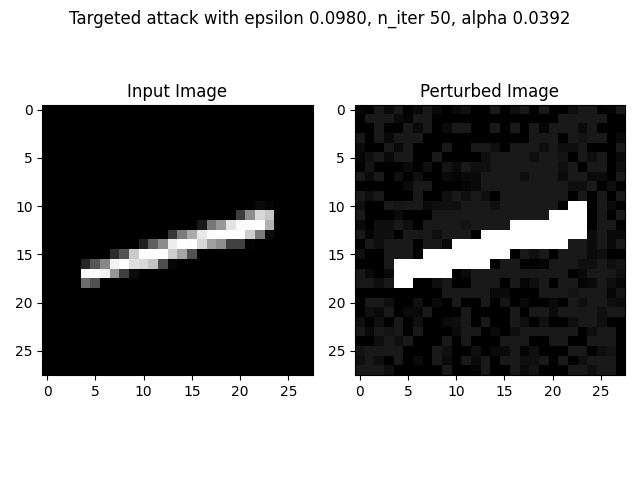
\includegraphics[trim={0 1.5cm 0cm 0}, width=.5\textwidth]{/Users/vashisth/Documents/GitHub/Intro_DL/IDL_HW3/HW3_tex/plots/Del6/Targeted/Targeted_attack__modA_e-0.0980_a-0.0392Img-2_iter50.png}
% \end{figure}
    \centering
    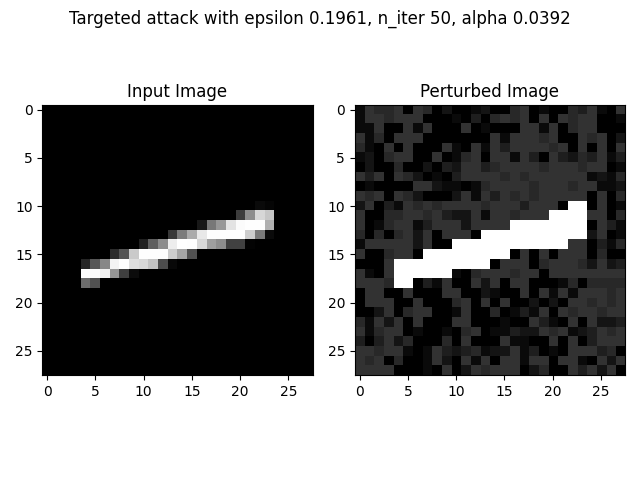
\includegraphics[trim={0 1.5cm 0cm 0}, width=.5\textwidth]{/Users/vashisth/Documents/GitHub/Intro_DL/IDL_HW3/HW3_tex/plots/Del6/Targeted/Targeted_attack__modA_e-0.1961_a-0.0392Img-2_iter50.png}
% \end{figure}
    \centering
    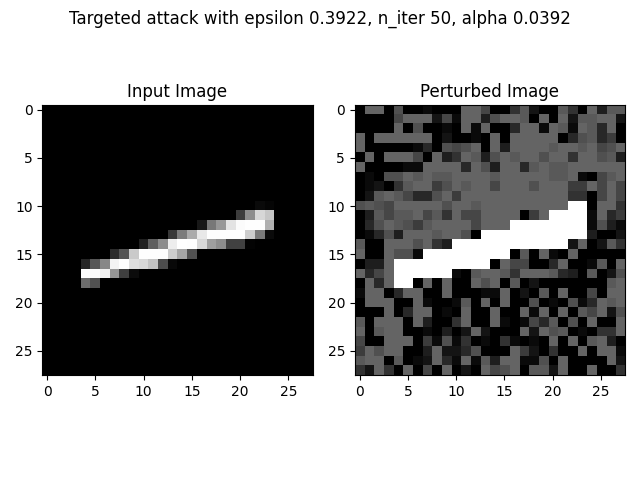
\includegraphics[trim={0 1.5cm 0cm 0}, width=.5\textwidth]{/Users/vashisth/Documents/GitHub/Intro_DL/IDL_HW3/HW3_tex/plots/Del6/Targeted/Targeted_attack__modA_e-0.3922_a-0.0392Img-2_iter50.png}
    \caption{Targeted Attack on Model A for Image with index 2 for different $\epsilon$}
\end{figure}



\begin{figure}[H]
    \centering
    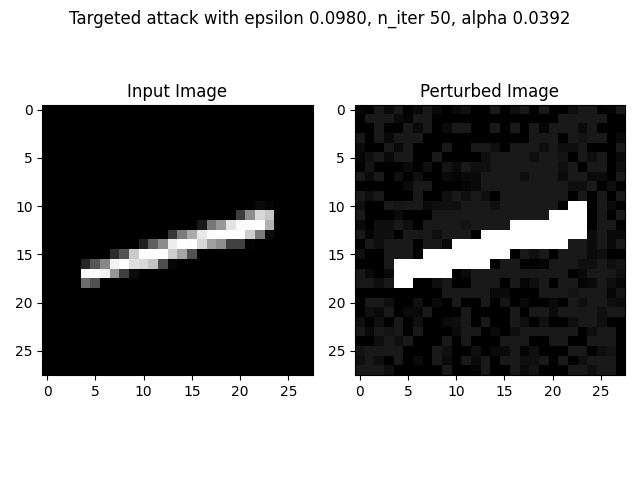
\includegraphics[trim={0 1.5cm 0cm 0}, width=.4\textwidth]{/Users/vashisth/Documents/GitHub/Intro_DL/IDL_HW3/HW3_tex/plots/Del6/Targeted/Targeted_attack__modA_e-0.0980_a-0.0392Img-2_iter50.png}
% \end{figure}
    \centering
    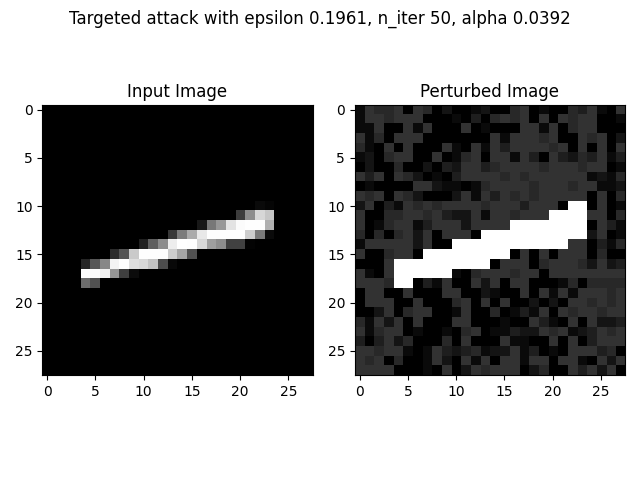
\includegraphics[trim={0 1.5cm 0cm 0}, width=.4\textwidth]{/Users/vashisth/Documents/GitHub/Intro_DL/IDL_HW3/HW3_tex/plots/Del6/Targeted/Targeted_attack__modA_e-0.1961_a-0.0392Img-2_iter50.png}
% \end{figure}
    \centering
    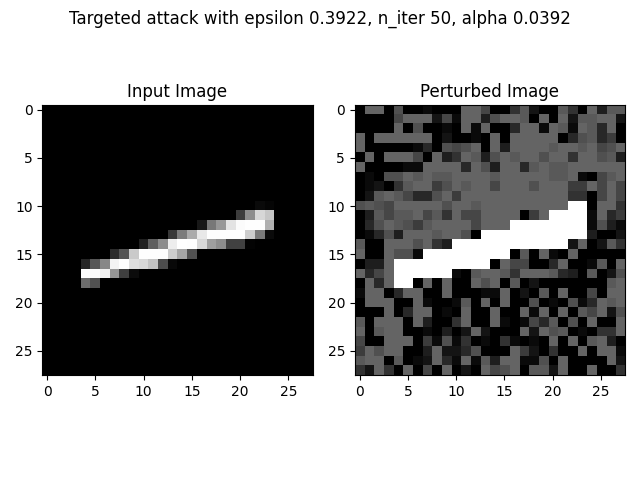
\includegraphics[trim={0 1.5cm 0cm 0}, width=.4\textwidth]{/Users/vashisth/Documents/GitHub/Intro_DL/IDL_HW3/HW3_tex/plots/Del6/Targeted/Targeted_attack__modA_e-0.3922_a-0.0392Img-2_iter50.png}
    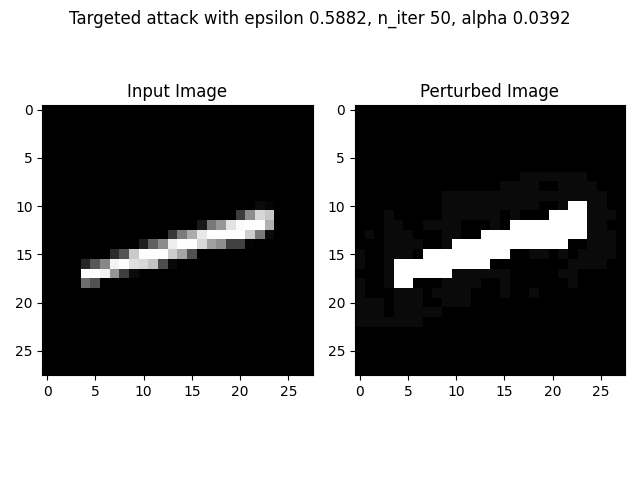
\includegraphics[trim = {0 1.5cm 0 0}, width = .4\textwidth] {/Users/vashisth/Documents/GitHub/Intro_DL/IDL_HW3/HW3_tex/plots/Del6/Targeted/Targeted_attack__modB_e-0.5882_a-0.0392Img-2_iter50.png}
    %%%%%
    \caption{Targeted Attack on Model B for Image with index 2 for different $\epsilon$ and $\alpha$ = 0.0392}
\end{figure}


\begin{figure}[H]
\centering
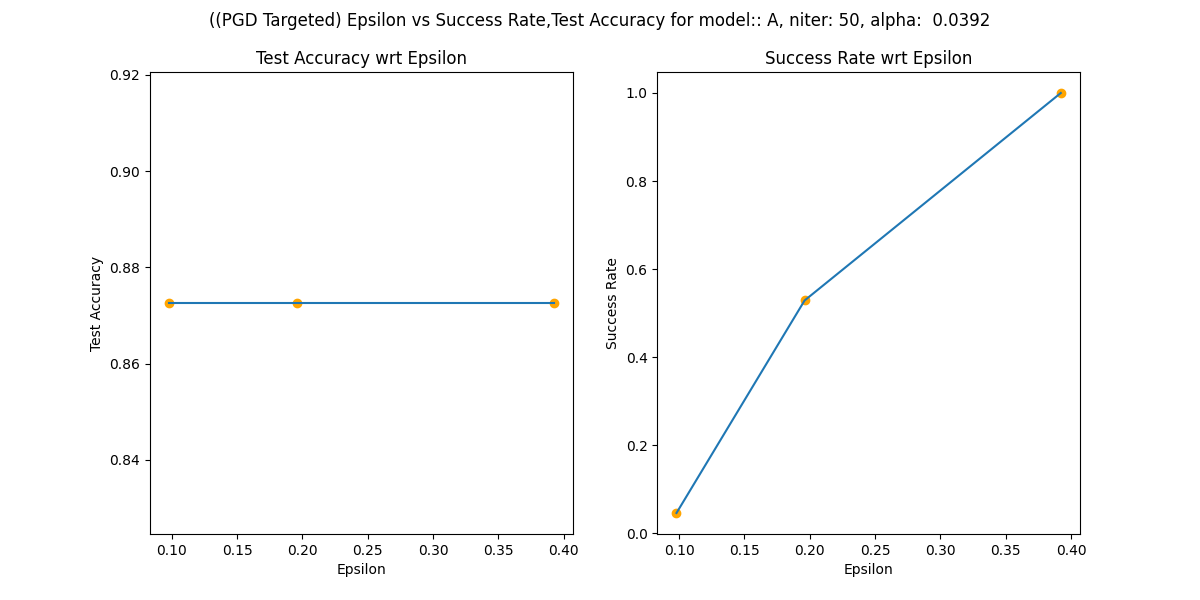
\includegraphics[width = .6 \textwidth]{/Users/vashisth/Documents/GitHub/Intro_DL/IDL_HW3/HW3_tex/plots/Del6/success_rate_plot_(PGD Targeted)_modA_iter50_a-0.0392.png}
\caption{Success Rate and Accuracy Plot for Targeted Attack on Model A}
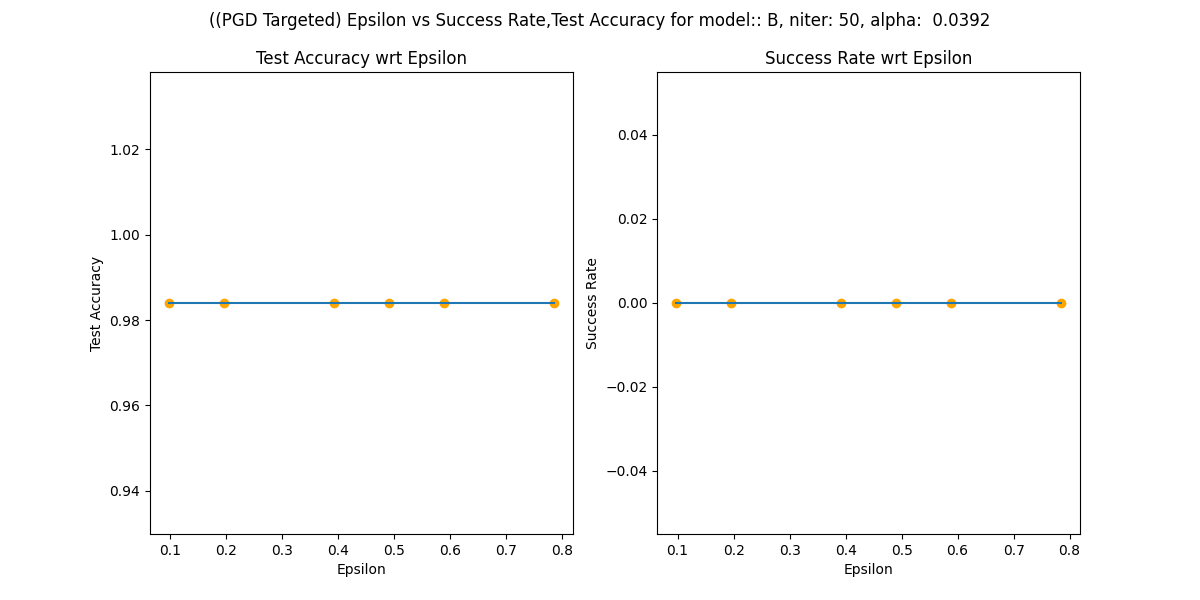
\includegraphics[width = .6 \textwidth]{/Users/vashisth/Documents/GitHub/Intro_DL/IDL_HW3/HW3_tex/plots/Del6/success_rate_plot_(PGD Targeted)_modB_iter50_a-0.0392.png}
\caption{Success Rate and Accuracy Plot for Targeted Attack on Model B}
\end{figure}

\end{solve}
%%%%%%%%%%%%%%%%%%%%%%%%%%%%%%%%%%%%%%%%%%%%%%%%%%%

% \subsubsection{Task 1 (Untargeted) vs Task 2 (Targeted)}


% \begin{solve}

% I am only showing this for one image here, but tried for a set of three images and the results were similar.

% The plots of purturbed images and the original images are shown below for both the tasks. The success rate and accuracy plots are also shown for both the models.

% Note that the success rate for Untargeted attacks just means that there was misclassificaiton, whereeas for Targeted attacks, it means that the attack was successful in making the model predict the target class (in our case our class that we want to attack was 1 and we wanted the model to predict 8). 

% We see that for epsilon .02 and .05 it is hard to see the difference between the original and the purturbed images, but for epsilon .1, the difference is visible. We start seeing artificats.

% Note that in the case of targeted attacks, we used PGD. Given the value of $\alpha = .0392$, we see that the attack is quite visible even for $\epsilon \sim .04$


% \textbf{Model A vs Model B}
% \begin{itemize}
%     \item For Untargeted attacks, the success rate is higher for Model B than Model A, it remains constant for Model B, but changes for Model A.
%     \item For Targeted attacks, the success rate is higher for Model A than Model B. This is because Model A is more accurate than Model B.
% \end{itemize}


% \subsubsection{Untargeted Attack}

% \begin{figure}[H]
%     \centering
%     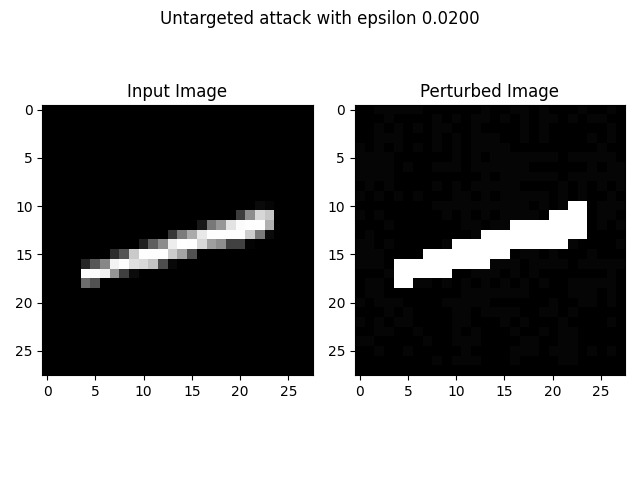
\includegraphics[trim={0 1.5cm 0cm 0}, width=.5\textwidth]{/Users/vashisth/Documents/GitHub/Intro_DL/IDL_HW3/HW3_tex/plots/Del6/Untargeted/Untargeted_attack__modA_0.0200_Img-2.png}
% % \end{figure}
% % \begin{figure}[H]
%     \centering
%     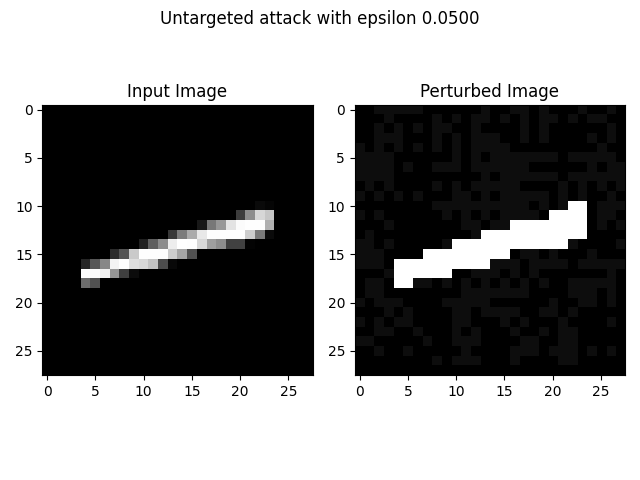
\includegraphics[trim={0 1.5cm 0cm 0}, width=.5\textwidth]{/Users/vashisth/Documents/GitHub/Intro_DL/IDL_HW3/HW3_tex/plots/Del6/Untargeted/Untargeted_attack__modA_0.0500_Img-2.png}
% % \end{figure}

% % \begin{figure}[H]
%     \centering
%     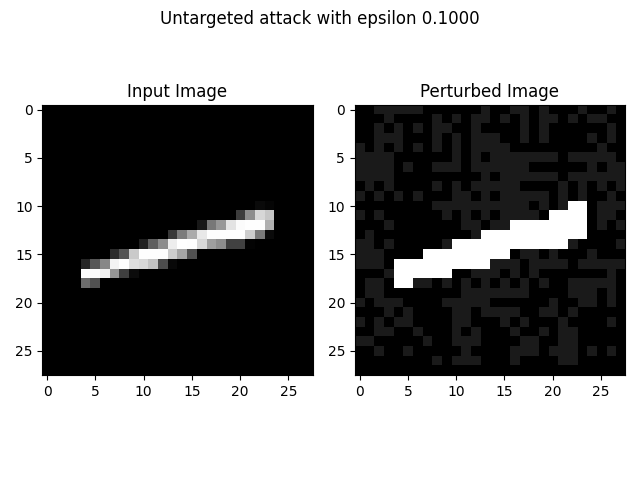
\includegraphics[trim={0 1.5cm 0cm 0}, width=.5\textwidth]{/Users/vashisth/Documents/GitHub/Intro_DL/IDL_HW3/HW3_tex/plots/Del6/Untargeted/Untargeted_attack__modA_0.1000_Img-2.png}
%     \caption{Untargeted Attack on Model A for Image with index 2 for different $\epsilon$}
% \end{figure}
% % [width = .99\textwidth]


% \begin{figure}[H]
%     \centering
%     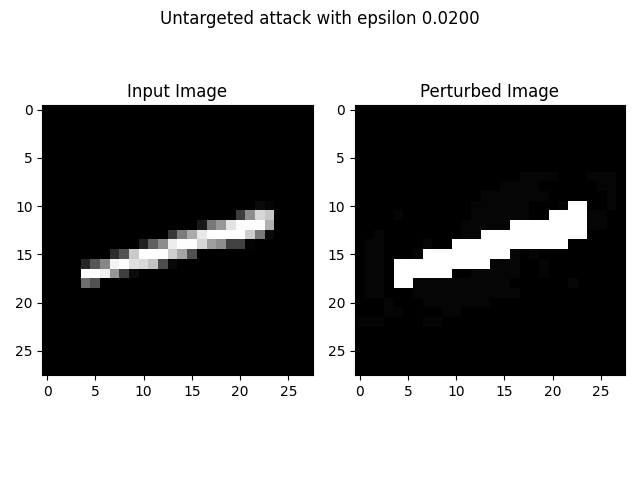
\includegraphics[trim={0 1.5cm 0cm 0}, width=.5\textwidth]{/Users/vashisth/Documents/GitHub/Intro_DL/IDL_HW3/HW3_tex/plots/Del6/Untargeted/Untargeted_attack__modB_0.0200_Img-2.png}
% % \end{figure}
% % \begin{figure}[H]
%     \centering
%     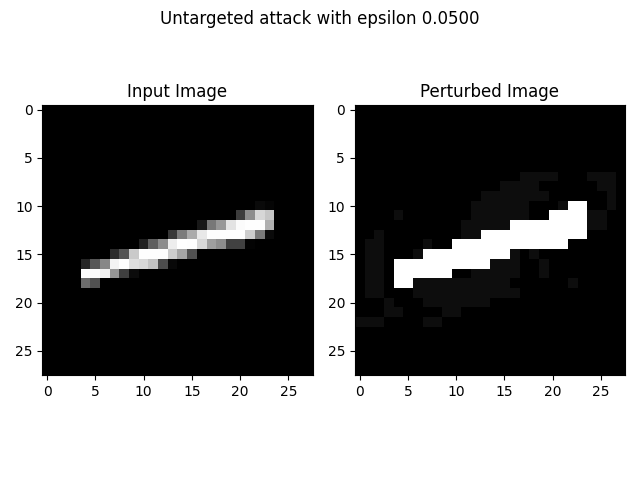
\includegraphics[trim={0 1.5cm 0cm 0}, width=.5\textwidth]{/Users/vashisth/Documents/GitHub/Intro_DL/IDL_HW3/HW3_tex/plots/Del6/Untargeted/Untargeted_attack__modB_0.0500_Img-2.png}
% % \end{figure}

% % \begin{figure}[H]
%     \centering
%     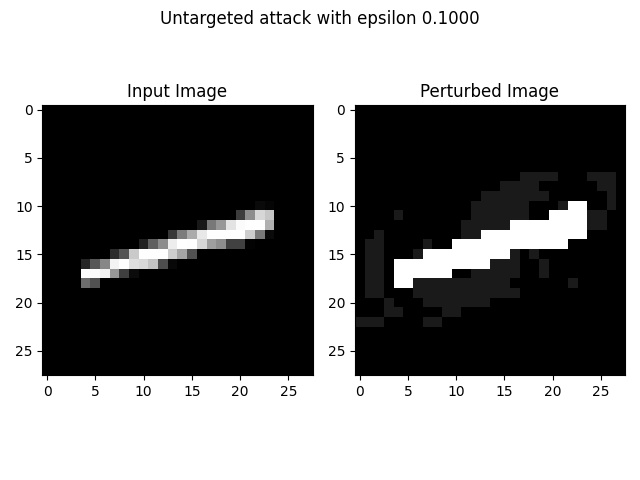
\includegraphics[trim={0 1.5cm 0cm 0}, width=.5\textwidth]{/Users/vashisth/Documents/GitHub/Intro_DL/IDL_HW3/HW3_tex/plots/Del6/Untargeted/Untargeted_attack__modB_0.1000_Img-2.png}
%     \caption{Untargeted Attack on Model B for Image with index 2 for different $\epsilon$}
% \end{figure}

% \begin{figure}[H]
% \centering
% 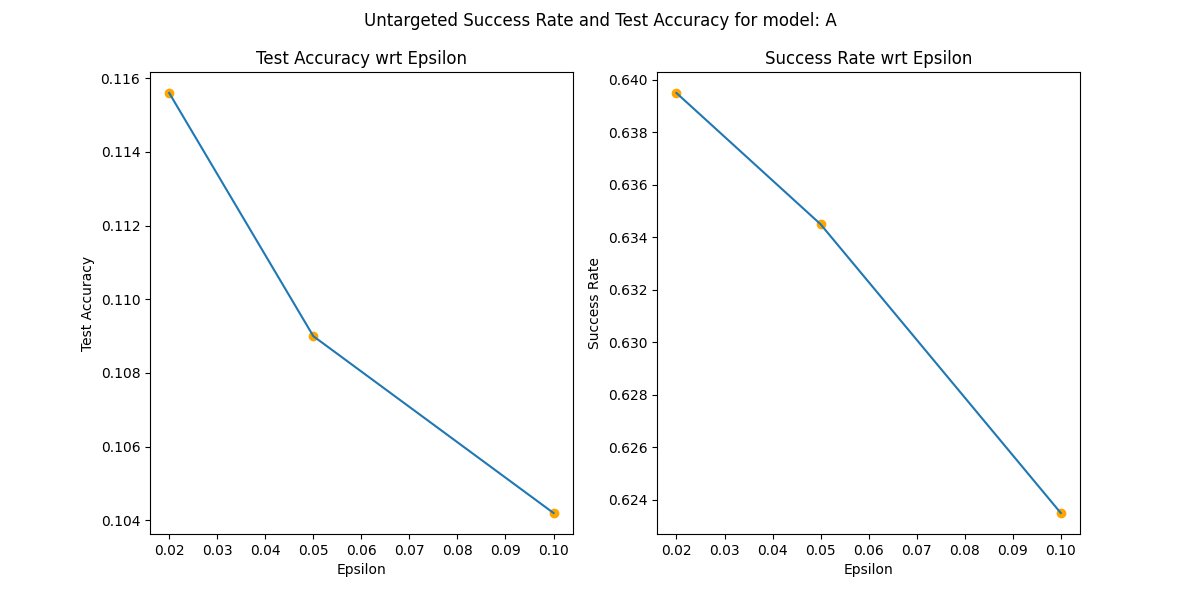
\includegraphics[width = .6 \textwidth]{/Users/vashisth/Documents/GitHub/Intro_DL/IDL_HW3/HW3_tex/plots/Del6/success_rate_plot_Untargeted_modA.png}
% \caption{Success Rate and Accuracy Plot for Untargeted Attack on Model A}
% 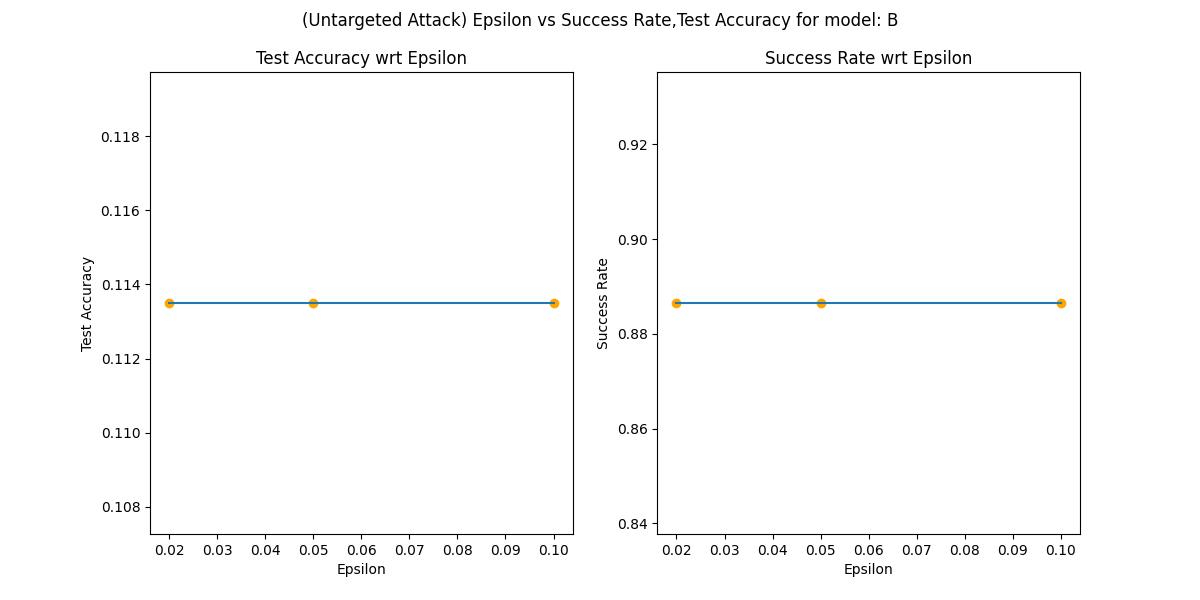
\includegraphics[width = .6 \textwidth]{/Users/vashisth/Documents/GitHub/Intro_DL/IDL_HW3/HW3_tex/plots/Del6/success_rate_plot_(Untargeted Attack)_modB.png}
% \caption{Success Rate and Accuracy Plot for Untargeted Attack on Model B}
% \end{figure}

% % \end{solve}


% %%%%%%%%%%%%%%%%%%%%%%%%%%%%%%%%%%%%%%%%%%

% \subsubsection{Targeted Attack}

% % \begin{solve}
% \begin{figure}[H]
%     \centering
%     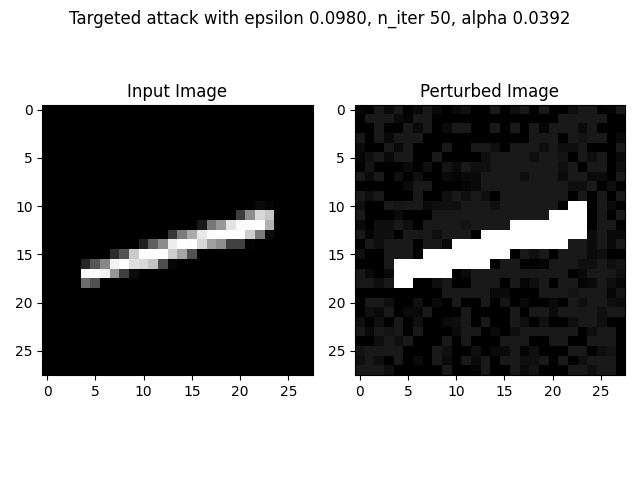
\includegraphics[trim={0 1.5cm 0cm 0}, width=.5\textwidth]{/Users/vashisth/Documents/GitHub/Intro_DL/IDL_HW3/HW3_tex/plots/Del6/Targeted/Targeted_attack__modA_e-0.0980_a-0.0392Img-2_iter50.png}
% % \end{figure}
%     \centering
%     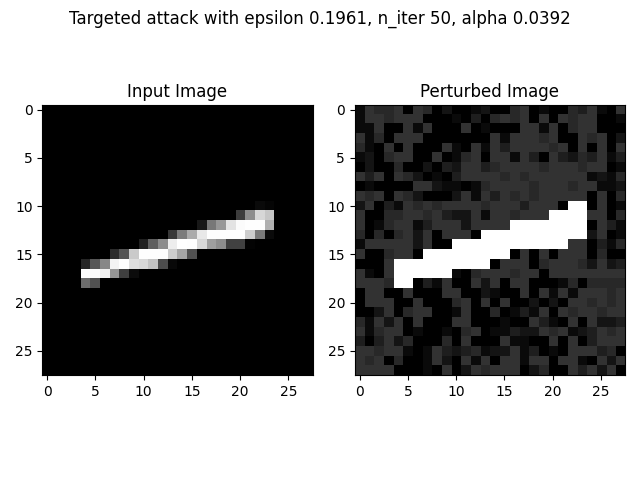
\includegraphics[trim={0 1.5cm 0cm 0}, width=.5\textwidth]{/Users/vashisth/Documents/GitHub/Intro_DL/IDL_HW3/HW3_tex/plots/Del6/Targeted/Targeted_attack__modA_e-0.1961_a-0.0392Img-2_iter50.png}
% % \end{figure}
%     \centering
%     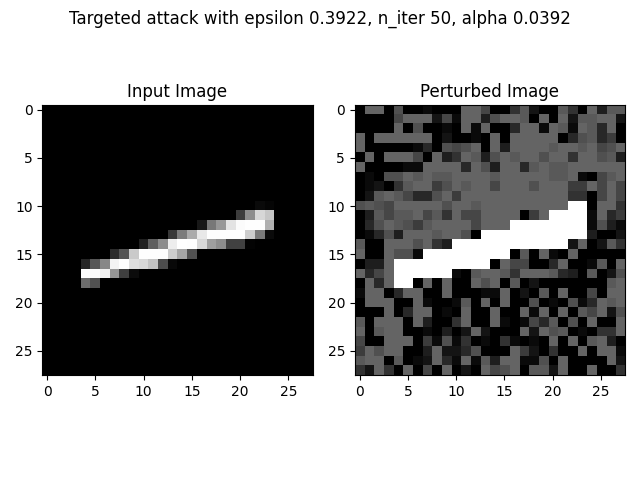
\includegraphics[trim={0 1.5cm 0cm 0}, width=.5\textwidth]{/Users/vashisth/Documents/GitHub/Intro_DL/IDL_HW3/HW3_tex/plots/Del6/Targeted/Targeted_attack__modA_e-0.3922_a-0.0392Img-2_iter50.png}
%     \caption{Targeted Attack on Model A for Image with index 2 for different $\epsilon$}
% \end{figure}



% \begin{figure}[H]
%     \centering
%     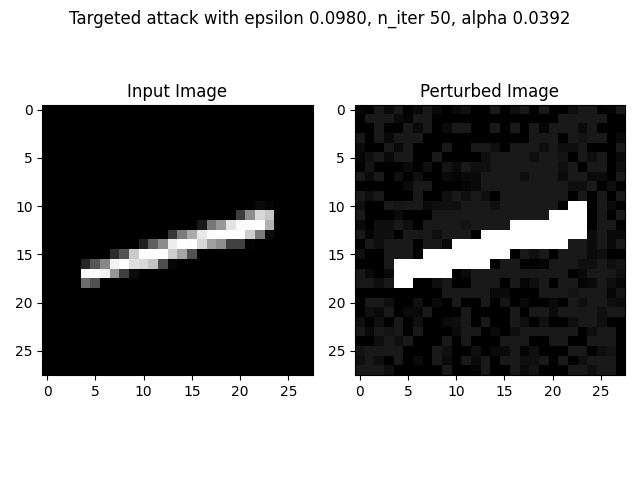
\includegraphics[trim={0 1.5cm 0cm 0}, width=.4\textwidth]{/Users/vashisth/Documents/GitHub/Intro_DL/IDL_HW3/HW3_tex/plots/Del6/Targeted/Targeted_attack__modA_e-0.0980_a-0.0392Img-2_iter50.png}
% % \end{figure}
%     \centering
%     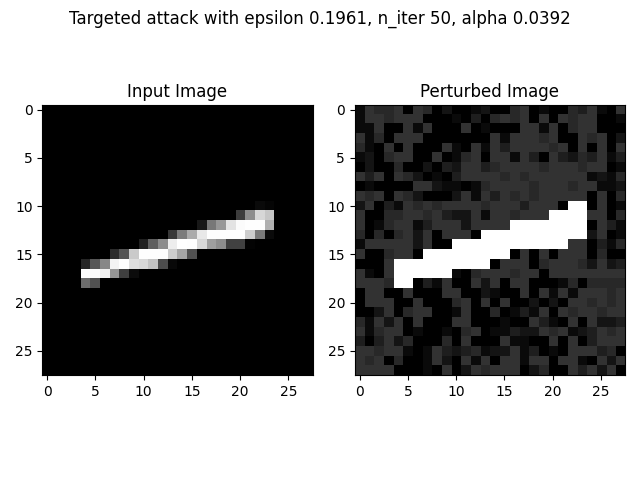
\includegraphics[trim={0 1.5cm 0cm 0}, width=.4\textwidth]{/Users/vashisth/Documents/GitHub/Intro_DL/IDL_HW3/HW3_tex/plots/Del6/Targeted/Targeted_attack__modA_e-0.1961_a-0.0392Img-2_iter50.png}
% % \end{figure}
%     \centering
%     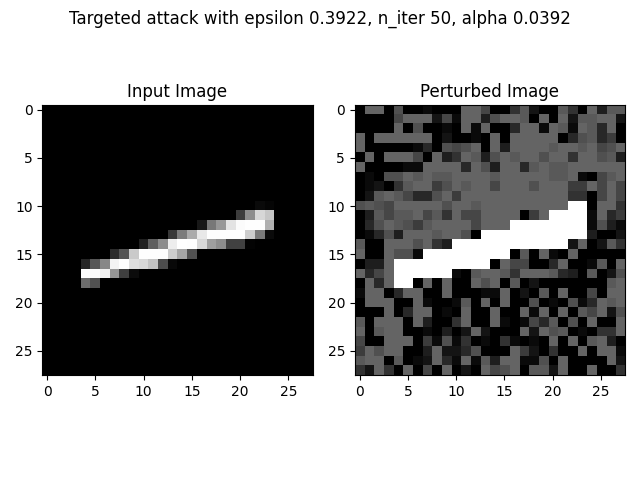
\includegraphics[trim={0 1.5cm 0cm 0}, width=.4\textwidth]{/Users/vashisth/Documents/GitHub/Intro_DL/IDL_HW3/HW3_tex/plots/Del6/Targeted/Targeted_attack__modA_e-0.3922_a-0.0392Img-2_iter50.png}
%     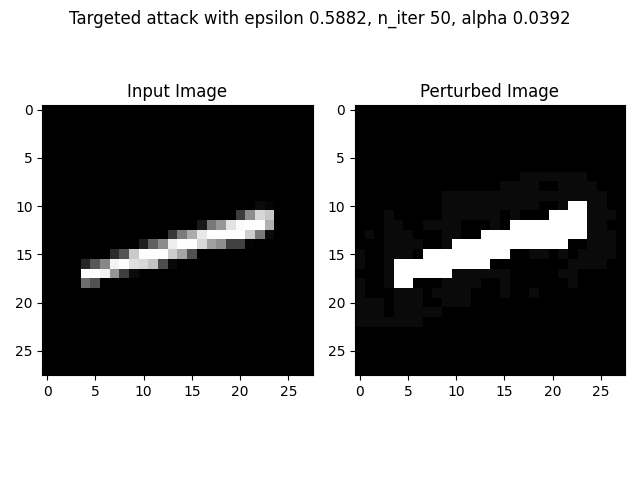
\includegraphics[trim = {0 1.5cm 0 0}, width = .4\textwidth] {/Users/vashisth/Documents/GitHub/Intro_DL/IDL_HW3/HW3_tex/plots/Del6/Targeted/Targeted_attack__modB_e-0.5882_a-0.0392Img-2_iter50.png}
%     %%%%%
%     \caption{Targeted Attack on Model B for Image with index 2 for different $\epsilon$ and $\alpha$ = 0.0392}
% \end{figure}


% \begin{figure}[H]
% \centering
% 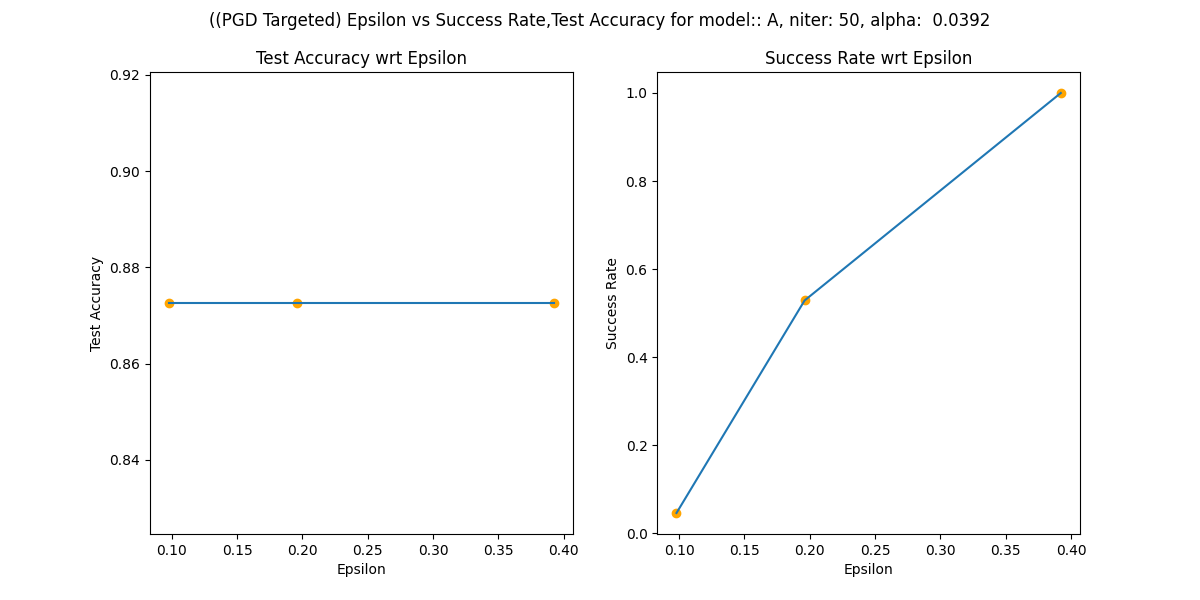
\includegraphics[width = .6 \textwidth]{/Users/vashisth/Documents/GitHub/Intro_DL/IDL_HW3/HW3_tex/plots/Del6/success_rate_plot_(PGD Targeted)_modA_iter50_a-0.0392.png}
% \caption{Success Rate and Accuracy Plot for Targeted Attack on Model A}
% 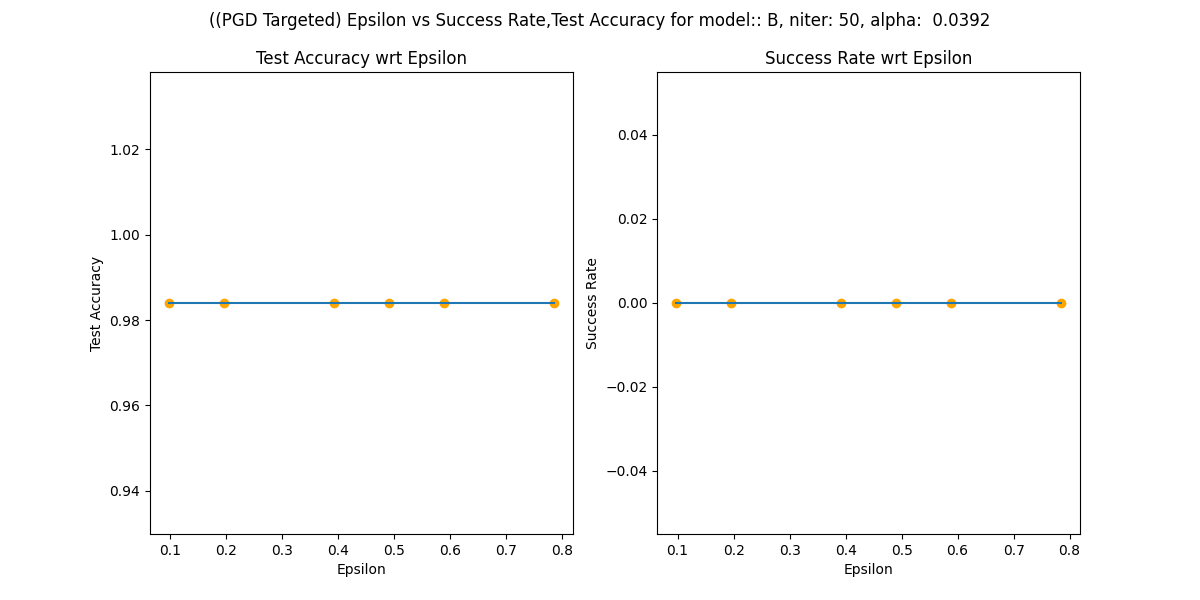
\includegraphics[width = .6 \textwidth]{/Users/vashisth/Documents/GitHub/Intro_DL/IDL_HW3/HW3_tex/plots/Del6/success_rate_plot_(PGD Targeted)_modB_iter50_a-0.0392.png}
% \caption{Success Rate and Accuracy Plot for Targeted Attack on Model B}
% \end{figure}

% \end{solve}
